\documentclass[11pt]{article}
\usepackage[utf8]{inputenc}
\usepackage{amsmath}
\usepackage{indentfirst}
\usepackage{graphicx}
\usepackage{subfigure}
\usepackage{float} 
\setlength{\parindent}{2em}
\usepackage{booktabs}
\usepackage{multirow}
\usepackage{geometry}
\usepackage{fancyhdr}
\pagestyle{fancy}
\fancyhf{}
\usepackage{xeCJK}
\usepackage{mathrsfs}
\usepackage{amsfonts,amssymb}
\usepackage{pdfpages}
\usepackage{bm}
\lhead{MATH1853: Linear Algebra}
\rhead{
\includegraphics[height = 0.75cm]{Auxiliary Files/Szgjzx-logo.png}}
\geometry{a4paper,scale=0.75}

\begin{document}
\section{Basic Concept}
\subsection{Fundamental Operations of Matrix}
If matrices $A$ and $B$ share the same numbers of column and row, then
\begin{gather}
    (A \pm B)_{ij} = A_{ij} \pm  B_{ij}\\
    (A B)_{ij} = \sum_{r=1}^{n}A_{1r}B_{rj} \\
    (A,~I) \sim (I,~A^{-1}) \\
    (A_1A_2\cdots A_n)^{T} = A_n^TA_{n-1}^T\cdots A_2^{T}A_1^{T}
\end{gather}
If $A_1,A_2,\dots,A_k$ are all $n \times n $ matrices, then
\begin{gather}
    (A_1A_2\dots A_k)^{-1} = A_k^{-1}A_{k-1}^{-1}\cdots A_2^{-1}A_1^{-1}
\end{gather}
If $\bm{x}$ is the solution to equation $A\bm{x} = \bm{b}$ or $\bm{x}A = \bm{b}$, then
\begin{equation}
    (A,~\bm{b}) \sim (I,~\bm{x})
\end{equation}
\subsection{Matrix and Linear Equations}
The following share the same solution:
\begin{equation}
\left\{
\begin{aligned}
    &\text{Matrix equation}~~A\bm{x}=\bm{b}\\
    &\text{Vector equation}~~\sum_{k=1}^{n}x_k\bm{a_k}=\bm{b}\\
    &\text{Augmented matrix}~~[\bm{a_1}~\bm{a_2}~\dots~\bm{a_n}~\bm{b}]\\
\end{aligned}
\right.
\end{equation}
There are three cases for the solution:
\begin{equation}
\left\{
\begin{aligned}
    &\text{Augmented matrix is not consistent} \rightarrow \bm{sol} = 0\\
    &\text{No free variable} \rightarrow \bm{sol} = 1~\text{(trivial solution)}\\
    &\text{Free variable exists} \rightarrow \bm{sol} = \text{infinite many}\\
\end{aligned}
\right.
\end{equation}
\subsection{Linearity}
\noindent \textbf{Theorem 1.3.1} If $A$ is an $m \times n $ matrix, the following propositions are equivalent
\begin{equation}
\boxed{\begin{aligned}
    &\text{a. for every $\bm{b}$ in $\mathbb{R}^m$, $A\bm{x} = \bm{b}$ has at least one solution}\\
    &\text{b. $\bm{Span}\{a_1, \dots, a_n\} = \mathbb{R}^m$}\\
    &\text{c. The columns of $A$ generate $\mathbb{R}^m$}\\
    &\text{d. $A$ has a pivot position in every row} \notag
\end{aligned}}
\end{equation}
\textbf{Theorem 1.3.2} If the columns of $A$ are linear independent, then the matrix equation $A\bm{x} = \bm{0}$ only have trivial solution. \par
\noindent \textbf{Theorem 1.3.3} If a mapping $x \mapsto T(x)$ is linear, then it is a closure.
\section{Homogeneous Coordinate}
\subsection{Method}
When translating a transform(compression, stretching, translation, rotation and perspective projection) of a graph into a matrix, we raise the coordinate to a higher dimension, i.e. $\mathbb{R}^{n} \rightarrow \mathbb{R}^{n+1}$. That is
\begin{equation}
    (x_1,x_2,\dots,x_n) \rightarrow (x_1,x_2,\dots,x_n,1)
\end{equation}
Then we can use a $(n+1)\times(n+1)$ matrix $A$ to represent the transform. \textbf{$\bm{A}$ can be considered as a set of the transform matrix applied on every basis of the homogeneous coordinate}.
\subsection{Implementation}
\subsubsection{Compression and Stretching}
\begin{equation}
    (x_1,x_2,\dots,x_n,1) \rightarrow (r_1x_1,r_2x_2,\dots,r_nx_n,1),~~
A=
\begin{bmatrix}
    r_1 &  &  & &\\
     & r_2 &  & &\\
     &  & r_3 &  &\\
     &  &  & \ddots & \\
     &  &  &  & 1\\
\end{bmatrix}
\end{equation}
\subsubsection{Translation}
If the translation vector $\bm{p} = (p_1, p_2, \dots, p_n)$, then
\begin{equation}
    (x_1, x_2, \dots, x_n, 1) \rightarrow (x_1+p_1, x_2+p_2, \dots, x_n+p_n, 1),~~A =
    \begin{bmatrix}
        1 &  &  &  &  & p_1\\
         & 1 &  & &  & p_2\\
         &  & 1 &  &  & p_3\\
         &  &  & \ddots &  &  \vdots\\
         &  &  &  & 1 & p_n\\
         &  &  &  &  & 1\\
    \end{bmatrix}
\end{equation}
\subsubsection{Rotation}
The axis around which a point $(x,y,z)$ rotates is denoted as $\bm{n}$, where
\begin{equation}
    \bm{n} = \begin{bmatrix}
    n_{x}  \\
    n_{y} \\
    n_{z} \\
    \end{bmatrix}
    ,~~n_{x}^2 + n_{y}^2 + n_{z}^2 = 1
\end{equation}
\begin{minipage}[b]{0.65\linewidth}
\begin{equation}
\begin{aligned}
    \bm{\omega} &= \bm{v_{\perp}}\times \bm{n} \\
    &=  \bm{v} \times \bm{n} \notag
\end{aligned}
\end{equation}
\begin{gather}
    \bm{v_{\parallel}} = (\bm{v}\cdot\bm{n})\bm{n} \notag,~~~\bm{v_{\parallel}} + \bm{v_{\perp}} = \bm{v} \\
    \bm{v_{\perp}'} = \bm{v_{\perp}} \text{cos}\theta + \bm{\omega}\text{sin}\theta = (\bm{v}-(\bm{v}\cdot \bm{n})\bm{n})\text{cos}\theta + (\bm{v} \times \bm{n} )\text{sin}\theta \notag \\
    \bm{v'} = \bm{v_{\perp}'} + \bm{v_{\parallel}'} = (\bm{v} \times \bm{n})\text{sin}\theta + (\bm{v}-(\bm{v}\cdot \bm{n})\bm{n})\text{cos}\theta + (\bm{v}\cdot \bm{n})\bm{n} \notag
\end{gather}
\end{minipage}
\hfill
\begin{minipage}[b]{0.55\linewidth}
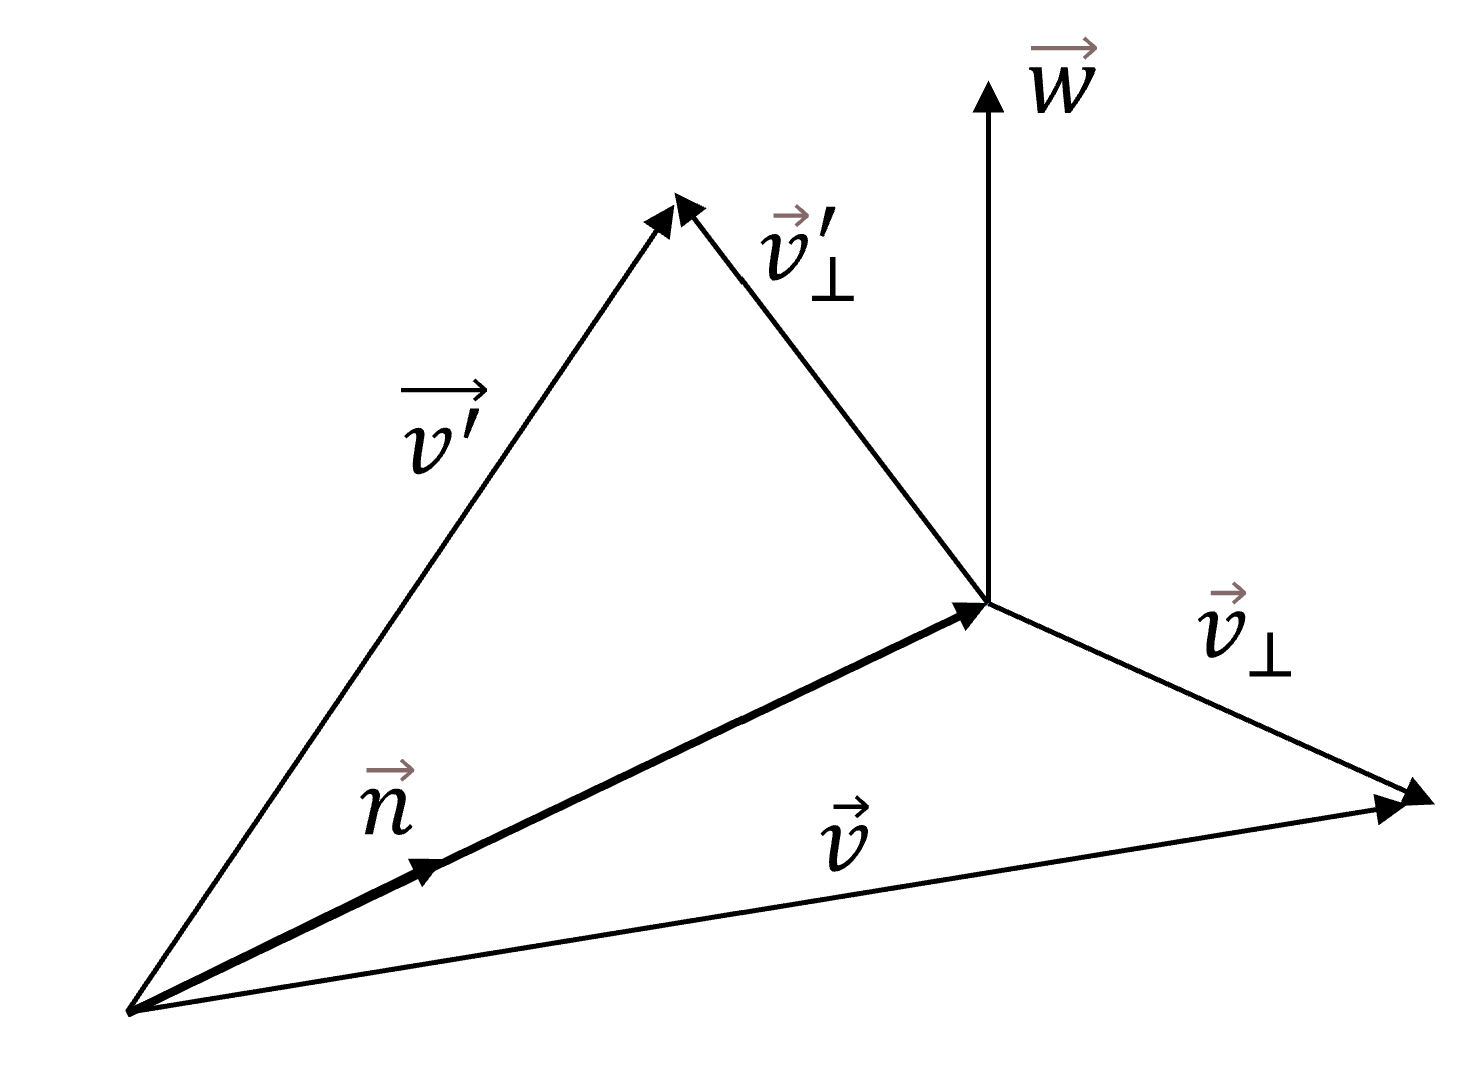
\includegraphics[height=8\baselineskip]{Auxiliary Files/Rotation Display.png}
\end{minipage}
Substitute in we obtain
\begin{equation}
\begin{aligned}
    \bm{v'} = \begin{bmatrix}
    x'\\ y' \\ z' \\
    \end{bmatrix} &= \text{sin}\theta \begin{bmatrix}
    n_{z}y-n_{y}z \\
    n_{x}z-n_{z}x \\
    n_{y}x-n_{x}y \\
    \end{bmatrix}
    + \text{cos}\theta 
    \left( \begin{bmatrix}
    x \\ y \\ z \\
    \end{bmatrix} -
    \begin{bmatrix}
    n_{x} \\ n_{y} \\ n_{z} \\
    \end{bmatrix}
    (n_{x}x + n_{y}y + n_{z}z) \right)
     + 
    \begin{bmatrix}
    n_{x} \\ n_{y} \\ n_{z} \\
    \end{bmatrix}
    (n_{x}x + n_{y}y + n_{z}z) \\
    &= \begin{bmatrix}
    (n_{x}^2 (1-\text{cos}\theta) +\text{cos}\theta )x + (n_{x}n_{y}(1-\text{cos}\theta) + n_{z}\text{sin}\theta ) y + (n_{x}n_{z} (1-\text{cos}\theta) - n_{y}\text{sin}\theta )z \\
    (n_{y}n_{z}(1-\text{cos}\theta) - n_{z}\text{sin}\theta)x + (n_{y}^2 (1-\text{cos}\theta) + \text{cos}\theta )y + (n_{z}n_{y}(1- \text{cos}\theta) + n_{x}\text{sin}\theta)z \\
    (n_{x}n_{z}(1-\text{cos}\theta) + n_{y}\text{sin}\theta)x + (n_{y}n_{z}(1-\text{cos}\theta) - n_{x}\text{sin}\theta)y + (n_{z}^2(1-\text{cos}\theta) + \text{cos}\theta)z
    \end{bmatrix} \notag
\end{aligned}
\end{equation}
Then the transform matrix is
\begin{equation}
    A = \begin{bmatrix}
    n_{x}^2 (1-\text{cos}\theta) +\text{cos}\theta & n_{x}n_{y}(1-\text{cos}\theta) + n_{z}\text{sin}\theta &  n_{x}n_{z} (1-\text{cos}\theta) - n_{y}\text{sin}\theta \\
    n_{y}n_{z}(1-\text{cos}\theta) - n_{z}\text{sin}\theta & n_{y}^2 (1-\text{cos}\theta) + \text{cos}\theta & n_{z}n_{y}(1- \text{cos}\theta) + n_{x}\text{sin}\theta \\
    n_{x}n_{z}(1-\text{cos}\theta) + n_{y}\text{sin}\theta & n_{y}n_{z}(1-\text{cos}\theta) - n_{x}\text{sin}\theta & n_{z}^2(1-\text{cos}\theta) + \text{cos}\theta
    \end{bmatrix}
\end{equation}
\subsubsection{Perspective Projection}
We are interested in the matrix representing a projection with an arbitrary point $(x_0,y_0,z_0)$ as the observation point to an arbitrary plane. \par
\begin{minipage}[b]{0.65\linewidth}
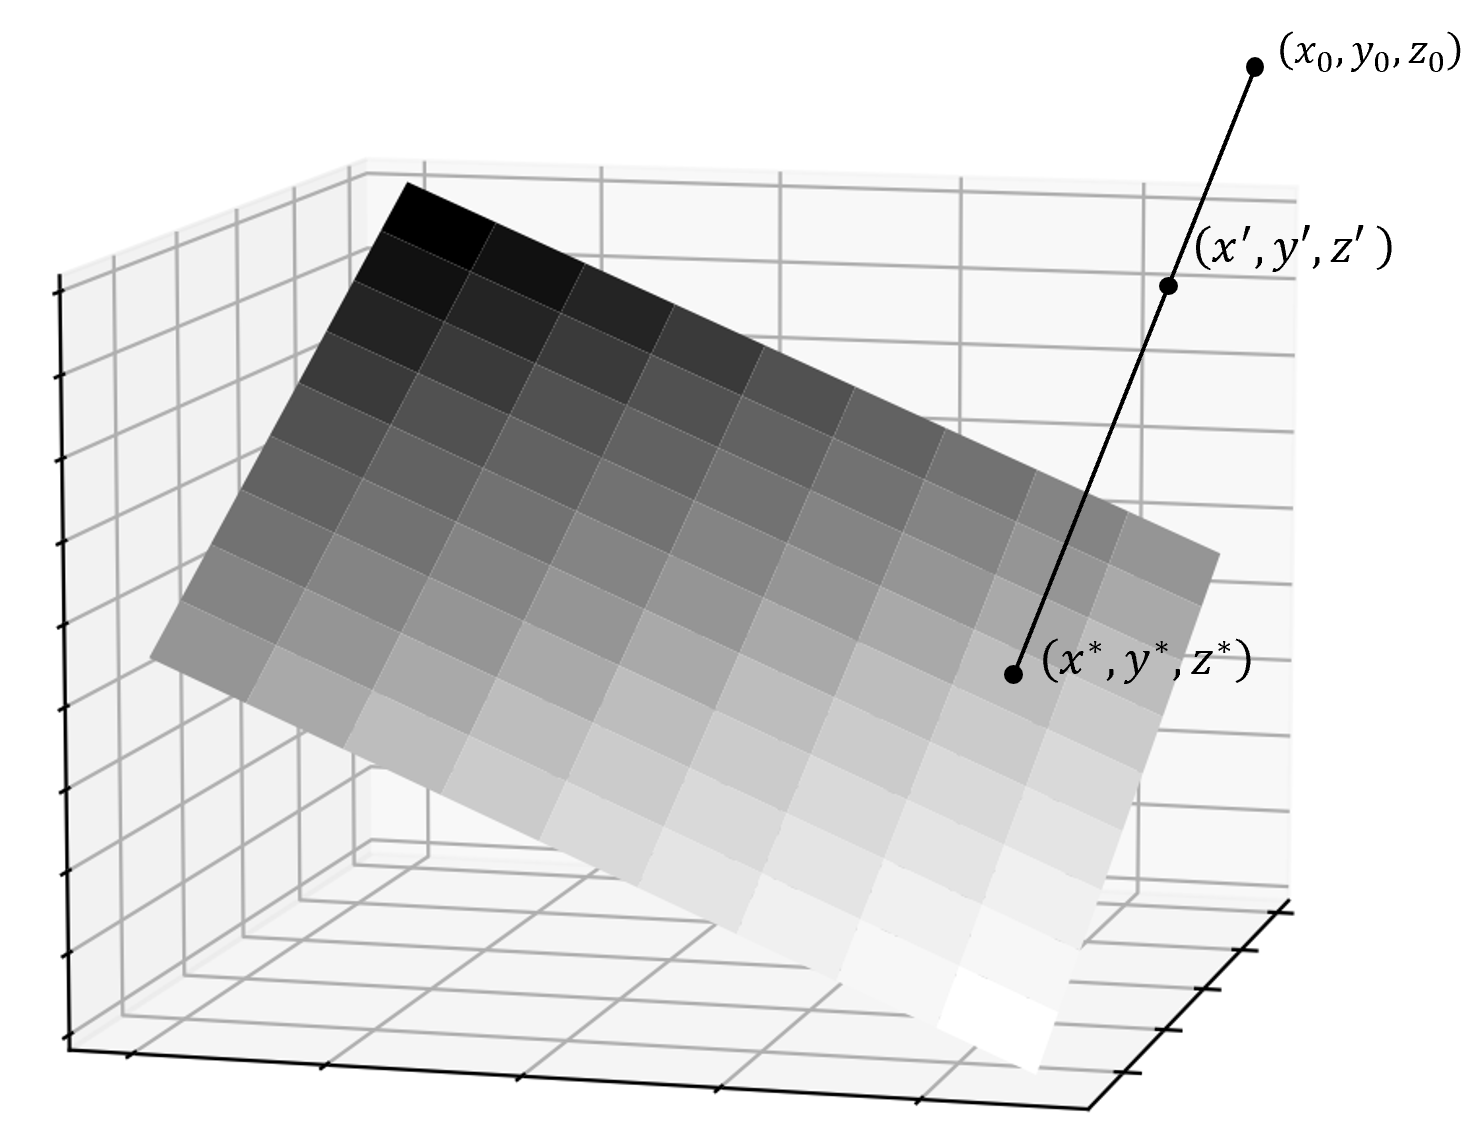
\includegraphics[height = 16\baselineskip]{Auxiliary Files/PLT.png}
\end{minipage}
\hfill
\begin{minipage}[b]{0.35\linewidth}
Equation of line:
\begin{equation}
    \frac{x-x_0}{x'-x_0} = \frac{y-y_0}{y'-y_0} = \frac{z-z_0}{z'-z_0} \notag
\end{equation}
Equation of plane:
\begin{equation}
    Ax+By+Cz+D=0 \notag
\end{equation}
\begin{equation}
    \rightarrow \left\{
    \begin{aligned}
        &Ax^* + By^*+Cz^*+D=0\\
        &x^*=(x'-x_0)k+x_0\\
        &y^*=(y'-y_0)k+y_0\\
        &z^*=(z'-z_0)k+z_0\\
    \end{aligned}
    \right.
\end{equation}
\end{minipage}
\par \indent \par
Solving (14) we obtain
\begin{equation}
    \begin{bmatrix}
    x' \\ y' \\ z' \\ 1 \\
    \end{bmatrix} \rightarrow \begin{bmatrix}
    x^*\\y^*\\z^*\\1\\
    \end{bmatrix} =
    \begin{bmatrix}
    -(By_0+Cz_0+D)x' +Bx_0y' +Cx_0z'+Dx_0 \\
    Ay_0x'-(Ax_0+Cz_0+D)y'+Cy_0z'+Dy_0\\
    Az_0x'+Bz_0y'-(Ax_0+By_0+D)z'+Dz_0\\
    Ax'+By'+Cz'-(Ax_0+By_0+Cz_0)\\
    \end{bmatrix}
\end{equation}
Hence the projection matrix is
\begin{equation}
    A_{\text{projection}} = \begin{bmatrix}
    -By_0-Cz_0-D & Bx_0 & Cx_0 & Dx_0 \\
    Ay_0 & -Ax_0 - Cz_0 - D & Cy_0 & Dy_0 \\
    Az_0 & Bz_0 & -Ax_0 -By_0 - D & Dz_0 \\
    A & B & C & -Ax_0 - By_0 - Cz_0 \\
    \end{bmatrix}
\end{equation}
\section{Gaussian Elimination}
\noindent \textbf{Definition} The Gaussian Elimination is a manipulation applied on a definite matrix. It contains the following operations:
\begin{equation}
\left\{
\begin{aligned}
    &\text{\textbf{Multiplying}: Multiplying a row by a non-zero number} \\
    &\text{\textbf{Adding}: Adding the multiple of a row to another one} \\
    &\text{\textbf{Swapping}: Exchanging the position of two definite rows}\\
\end{aligned}
\right.
\end{equation}
The result of applying the Gaussian Elimination is generating a row echelon form, denoted as matrix $U$. $A$ and $U$ are row equivalent, i.e. $A \sim U$. For instance:
\begin{equation}
\begin{bmatrix}
    a_{11} & a_{12} & \cdots & a_{1n}\\
    a_{21} & a_{22} & \cdots & a_{2n}\\
    \vdots & \vdots & \ddots & \vdots\\
    a_{m1} & a_{m2} & \cdots & a_{mn}\\
\end{bmatrix}
\underrightarrow{\text{Gaussian Elimination }}
\begin{bmatrix}
    a'_{11} & a'_{12} & \cdots & a'_{1n}\\
     & a'_{22} & \cdots & a'_{2n} \\
     &  & \ddots & \vdots \\
     &  &  & a'_{mn}
\end{bmatrix}
\end{equation}
If in the transformation, we only use the \textbf{Adding} operation, which can be represented as $E_i$ at the $i$th step, then
\begin{equation}
    E_pE_{p-1}\cdots E_1A = U,~~\text{or}~L = (E_pE_{p-1}\cdots E_1)^{-1},~A = LU
\end{equation}
Where $L$ is an $m \times m$ unit lower triangular matrix, while $U$ is an $m \times n$ upper triangular matrix equivalent to $A$. We can conclude that
\begin{equation}
    (A,~L) \sim (U,~I)
\end{equation}
\section{Inverse of Matrix}
For an $n \times n$ matrix, its inverse is defined as
\begin{equation}
    A^{-1}:~~A^{-1}A = AA^{-1} = I_n
\end{equation}
\subsection{Criterion}
The invertibility of an arbitrary matrix can be judged by the following features:
\begin{equation}
    \boxed{\text{The columns of $A$ are linearly independent} \Leftrightarrow \text{The columns of $A$ is a basis of  $\mathbb{R}^n$} \Leftrightarrow \bm{det}A \neq 0} \notag
\end{equation}
\subsection{Proof}
If the columns of $A$ are linear dependent,
\begin{gather}
    \exists~a_i \in A,~\exists~\{c_1, c_2, \dots, c_{i-1}\},~a_i = \sum_{k=1}^{i-1}c_k a_k \notag \\
    A^{T} = \begin{bmatrix}
    a_1 & a_2 & \cdots & a_i & \cdots & a_n 
    \end{bmatrix}^{T} \sim
    \begin{bmatrix}
    a_1 & a_2 & \cdots & \bm{0} & \cdots & a_n
    \end{bmatrix}^{T} \notag
\end{gather}
Then
\begin{equation}
    \bm{det}A = \bm{det}A^{T}=\bm{det}\begin{bmatrix}
    a_1 & a_2 & \dots & \bm{0} & \dots & a_n
    \end{bmatrix}^{T} = 0 \notag
\end{equation}
And vice versa, QED
\section{Dimensions and Rank}
\subsection{Basis} 
\noindent \textbf{Definition} Given that $\mathcal{B} = \{b_1, b_2, \dots, b_p\}$ is a set of basis to linear space $H$, then for every vector $\bm{x}$ in $H$, there is a unique coordinate to represent it:
\begin{equation}
    \bm{[x]_{\mathcal{B}}} = [c_1, c_2, \dots, c_p]^{T},~~\bm{x} = [\mathcal{B}]\bm{[x]_{\mathcal{B}}}
\end{equation}
A set of basis should be linear independent, i.e. equation $[\mathcal{B}]x = \bm{0}$ has only trivial solution. \textbf{Particularly, the rows of an \underline{echelon form} are linear independent} \par \indent \par
\noindent \textbf{Theorem 5.1.1} Given that $A$ is a matrix and its echelon form is $U$, the non-zero rows of $U$ are the basis of $\bm{\text{\textbf{Row}}A}$, while the corresponding columns to the pivot columns of $U$ in $A$ are the basis of $\bm{\text{\textbf{Col}}A}$ .
\subsection{Dimension}
\noindent \textbf{Definition} The dimension of a linear space $V$ is the number of vectors its arbitrary basis contains, denoted as $\bm{\text{\textbf{dim}}V}$.
\begin{equation}
    \mathcal{B} = \{b_1, b_2, \dots, b_p\},~b_1,b_2,\dots,b_p \in V~ \rightarrow~\text{dim}V = p \notag
\end{equation}
For finite dimensional space, $p$ is an integer. Particularly, for an infinite dimensional space $V$, $\text{dim}V = \infty$.
\subsection{Rank}
The rank of an $m \times n$ matrix $A$ is the dimension of its column space, denoted as $\text{rank}A$.
\begin{equation}
    \text{rank}A + \text{dim}~\text{Nul}A = n
\end{equation}
\section{Inverse of Block Matrix}
We are interested in the inverse of a $2\times 2$ block matrix $T$, denoted as
\begin{equation}
    T = \begin{bmatrix}
    \bm{A_{11}} & \bm{A_{12}} \\ \bm{A_{21}} & \bm{A_{22}}
    \end{bmatrix}
\end{equation}
Assume that the left-upper block $\bm{A_{11}}$ is invertible, then denote the inverse matrix as $T^{-1}$, where
\begin{equation}
    T^{-1} = \begin{bmatrix}
    \bm{B_{11}} & \bm{B_{12}} \\ \bm{B_{21}} & \bm{B_{22}}
    \end{bmatrix}
\end{equation}
From the definition $TT^{-1} = \bm{I}$, we have
\begin{equation}
    \left\{
    \begin{aligned}
        &\bm{A_{11}} \bm{B_{11}} + \bm{A_{12}}\bm{B_{21}} = \bm{I} \\
        &\bm{A_{11}} \bm{B_{12}} + \bm{A_{12}}\bm{B_{22}} = \bm{0} \\
        &\bm{A_{21}} \bm{B_{11}} + \bm{A_{22}} \bm{B_{21}} = \bm{0} \\
        &\bm{A_{21}} \bm{B_{12}} + \bm{A_{22}} \bm{B_{22}} = \bm{I} 
    \end{aligned}
    \right.
\end{equation}
We take steps to solve the equations system.
\begin{equation}
    \left\{ \begin{aligned}
        &\bm{B_{12}} + \bm{A_{11}}^{-1} \bm{A_{12}}\bm{B_{22}} = \bm{0} \\
        &\bm{A_{21}} \bm{B_{12}} + \bm{A_{22}} \bm{B_{22}} = \bm{I}
    \end{aligned}
    \right.~\rightarrow~\bm{B_{22}} = (\bm{A_{22}} - \bm{A_{21}}\bm{A_{11}^{-1}} \bm{A_{12}})^{-1} = \bm{F},~~\bm{B_{12}} = -\bm{A_{11}}^{-1}\bm{A_{22}}\bm{F} \notag
\end{equation}
\begin{equation}
\left\{ \begin{aligned}
    &\bm{B_{11}} + \bm{A_{11}}^{-1}\bm{A_{12}}\bm{B_{21}} = \bm{A_{11}}^{-1} \\
    &\bm{A_{21}}\bm{B_{11}} + \bm{A_{22}}\bm{B_{21}} = \bm{0}
\end{aligned} \right.~\rightarrow~\begin{aligned}\bm{B_{21}} &= -(\bm{A_{22}} - \bm{A_{21}}\bm{A_{11}}^{-1}\bm{A_{12}})^{-1} \bm{A_{21}}\bm{A_{11}}^{-1} = -\bm{F}\bm{A_{21}}\bm{A_{11}}^{-1} \\ 
\bm{B_{11}} &=  \bm{A_{11}}^{-1}-\bm{A_{11}}^{-1}\bm{A_{12}}\bm{B_{21}} = \bm{A_{11}}^{-1}(\bm{I} + \bm{A_{12}}\bm{F} \bm{A_{21}}\bm{A_{11}}^{-1}) \notag
\end{aligned}
\end{equation}
Hence we can conclude that the inverse matrix is
\begin{equation}
    T^{-1} = \begin{bmatrix}
    \bm{A_{11}}^{-1}(\bm{I} + \bm{A_{12}}\bm{F} \bm{A_{21}}\bm{A_{11}}^{-1}) &  -\bm{A_{11}}^{-1}\bm{A_{22}}\bm{F}  \\
    -\bm{F}\bm{A_{21}}\bm{A_{11}}^{-1} & \bm{F}
    \end{bmatrix}~~~~~\bm{F} = (\bm{A_{22}} - \bm{A_{21}}\bm{A_{11}^{-1}} \bm{A_{12}})^{-1}
\end{equation}
\section{Cramer's Rule}
\subsection{Content}
If the linear equation $Ax = c$ has solution vector $x = (x_1, x_2,\dots, x_n)^{T}$.Then the solution $x_i$ is
\begin{equation}
    x_i = \frac{\bm{det}A_i(c)}{\bm{det}A}
\end{equation}
where $A_i$ is the resultant matrix by replacing the $i$th column of the original matrix by column vector $c$.
\subsection{Proof}
Given that $Ax = c$, then
\begin{equation}
    A^{-1}Ax = A^{-1}c = Ix = x
\end{equation}
We are interested in $\bm{det}A_i$, that is
\begin{equation}
\begin{aligned}
    \bm{det}A_i(c) &= \bm{det}(a_1, a_2, \dots, a_{i-1}, c, a_{i+1}, \dots, a_{n-1}, a_n)\\
    &= \bm{det}(a_1, a_2, \dots, a_{i-1}, \sum^{n}_{k=1}x_ka_k, a_{i+1}, \dots, a_{n-1}, a_n)\\
    &= \sum_{k=1}^{n} x_k~\bm{det}(a_1,a_2,\dots,a_{i-1},a_k, a_{i+1}, \dots, a_{n-1}, a_n)
\end{aligned}
\end{equation}
With the alternative feature of determinant, we have
\begin{gather}
    \bm{det}(u_1, u_2, \dots, u_i, \dots, u_j, \dots, u_n) = -\bm{det}(u_1, u_2, \dots, u_j, \dots, u_i, \dots, u_n) \\
    \exists~\text{i, j},~i\neq j,~u_i = u_j,~u_i,~u_j \in A~~\rightarrow~~\bm{det}A = 0
\end{gather}
Then the equation in (6) gives
\begin{gather}
    \sum_{k=1}^{n} x_k~\bm{det}(a_1,a_2,\dots,a_{i-1},a_k, a_{i+1}, \dots, a_{n-1}, a_n) = x_i~\bm{det}(a_1, a_2, \dots, a_n) \notag \\
    \bm{det}A_i(c) = x_i~\bm{det}A~~~~\text{QED}
\end{gather}
\subsection{Application}
A significant application of Cramer's Rule is to give a simplified calculation for the inverse to a square matrix. To find an inverse, we may consider the following matrix equation.
\begin{equation}
    AA^{-1} = I,~~~~\text{or}~~    \bigoplus_{j=1}^{n}AA^{-1}_{j} = \bigoplus_{j=1}^{n}e_{j}
\end{equation}
Where $A^{-1}_j$ and $I_{j}$ represents the $j$th column of $A^{-1}$ and $I$ respectively. Then we treat every column of $A^{-1}$ as the solution to equation
\begin{equation}
    A\bm{x} = e_j
\end{equation}
Applying Cramer's rule,
\begin{equation}
\begin{aligned}
    x_i &= \frac{\bm{det}A_i(e_j)}{\bm{det}A} \\
    &= \frac{1}{\bm{det}A} \cdot \bm{det}
    \begin{bmatrix}
    a_{1,1} & a_{1,2} & \cdots & a_{1,i-1} & 0 & a_{1,i+1} & \cdots & a_{1,n} \\
    \vdots & \vdots & \ddots & \vdots & \vdots & \vdots & \ddots & \vdots \\
    a_{j,1} & a_{j,2} & \cdots & a_{j,i-1} & 1 & a_{j,i+1} & \cdots & a_{j, n} \\
    \vdots & \vdots & \ddots & \vdots & \vdots & \vdots & \ddots & \vdots \\
    a_{n,1} & a_{n,2} & \cdots & a_{n,i-1} & 0 & a_{n,i+1} & \cdots & a_{n,n}\\
    \end{bmatrix} \\
    &= \frac{1}{\bm{det}A} C_{j,i}
\end{aligned}
\end{equation}
\begin{equation}
    \bm{x} = \frac{1}{\bm{det}A} \begin{bmatrix}
    C_{j,1} & C_{j,2} & \cdots C_{j,n}
    \end{bmatrix}^{T}
\end{equation}
Then we can combine all the solutions to obtain the general solution
\begin{equation}
\begin{aligned}
    A^{-1} = \bigoplus_{j=1}^{n} \bm{x} &= \frac{1}{\bm{det}A} \begin{bmatrix}
    C_{1,1} & C_{2,1} & \cdots & C_{n,1} \\
    C_{1,2} & C_{2,2} & \cdots & C_{n,2} \\
    \vdots & \vdots & \ddots & \vdots \\
    C_{1,n} & C_{2,n} & \cdots & C_{n,n} \\
    \end{bmatrix}
    \\ &= \frac{1}{\bm{det}A}~\text{adj}A
\end{aligned}
\end{equation}
The matrix \textbf{adj}$\bm{A}$ is called the \underline{adjugate matrix} of $A$.
\section{Vandermonde Matrix}
\noindent \textbf{Definition} A Vandermonde matrix is an $m \times n$ matrix with geometric terms in each row, i.e.
\begin{equation}
    V = 
    \begin{bmatrix}
    & 1 & x_1 & x_1^2 & \cdots & x_1^{n-1}\\
    & 1 & x_2 & x_2^2 & \cdots & x_2^{n-1}\\
    & \vdots & \vdots & \vdots & \ddots & \vdots\\
    & 1 & x_m & x_m^2 & \cdots & x_m^{n-1}\\
    \end{bmatrix},~~
    \text{or}~~V_{i,j} = x_i^{j-1}
\end{equation}
The determinant of the matrix can be calculated as follows when $m = n$. A new matrix $V'$ can be defined such that
\begin{equation}
    V'_{i,j} = V_{i,j} - x_1V_{i,j-1},~~1\leq i,j \leq n
\end{equation}
\begin{equation}
    V' = 
    \begin{bmatrix}
    & 1 & 0 & 0 & \cdots & 0\\
    & 1 & x_2-x_1 & x_2(x_2-x_1) & \cdots & x_2^{n-2}(x_2-x_1)\\
    & 1 & x_3-x_1 & x_3(x_3-x_1) & \cdots & x_3^{n-2}(x_3-x_1)\\ 
    & \vdots & \vdots & \vdots & \ddots & \vdots\\
    & 1 & x_n-x_1 & x_n(x_n-x_1) & \cdots & x_n^{n-2}(x_n-x_1)\\
    \end{bmatrix}
\end{equation}
As $V'^{T}$ and $V^{T}$ are row equivalent, $\bm{det}V'= \bm{det}V$. Applying Laplace expansion on $V'$, we obtain
\begin{equation}
\begin{aligned}
    \bm{det}V' = \sum_{k=1}v'_{1,k}C_{1,k} &= v'_{1,1}\cdot \bm{det}B =     
    \begin{vmatrix}
    & x_2-x_1 & x_2(x_2-x_1) & \cdots & x_2^{n-2}(x_2-x_1)\\
    & x_3-x_1 & x_3(x_3-x_1) & \cdots & x_3^{n-2}(x_3-x_1)\\ 
    & \vdots & \vdots & \ddots & \vdots\\
    & x_n-x_1 & x_n(x_n-1) & \cdots & x_n^{n-2}(x_n-x_1)\\
    \end{vmatrix}\\
    &=\prod_{k=2}^{n}(x_k-x_1)
    \begin{vmatrix}
    &1 & x_2 & \cdots & x_2^{n-2}\\
    &1 & x_3 & \cdots & x_3^{n-2}\\
    &\vdots & \vdots & \ddots & \vdots\\
    &1 & x_n & \cdots & x_n^{n-2}
    \end{vmatrix}
\end{aligned}
\end{equation}
The determinant of an $m \times n$ has reduced to a $(n-1)\times(n-1)$ one. Recursively, we can conclude that
\begin{equation}
\begin{aligned}
    \bm{det}V  &= \prod_{k=2}^{n}(x_k-x_1) \prod_{k=3}^{n}(x_k-x_2) \cdots \prod_{k=n}^{n}(x_k-x_{n-1})\\
    &= \prod_{1\leq i < j \leq n }(x_j - x_i)
\end{aligned}
\end{equation}
\section{Eigenvalue and Eigenvector}
\subsection{Definition}
For an $n \times n$ matrix $A$, if
\begin{equation}
    \exists~\lambda,~~A\bm{x} = \lambda \bm{x}~\text{has non-trivial solution}
\end{equation}
In other words, $\text{Nul}(A-I\lambda) \neq \{\bm{0}\}$. $\lambda$ is defined as the \textbf{eigenvalue} of matrix $A$, while $\bm{x}$ is the eigenvector corresponds to $\lambda$.
\subsection{Linearity of Eigenvectors}
\noindent \textbf{Theorem 8.2.1}
if $\lambda_1, \lambda_2, \dots, \lambda_p$ are the mutually different eigenvalues of matrix $A$, and corresponds to eigenvectors $v_1, v_2, \dots, v_p$ respectively, then
\begin{equation}
    \{\bm{v_1}, \bm{v_2}, \dots, \bm{v_p}\}
\end{equation}
is a set of linearly independent vectors. \par \noindent
\textbf{Proof} If the set is linearly dependent, we obtain
\begin{equation}
    \exists~\bm{v_r} \in \{\bm{v_1}, \bm{v_2}, \dots, \bm{v_p}\},~~\sum_{k=1}^{r}c_{k}\bm{v_{k}} = \bm{v_{r+1}}
\end{equation}
Then
\begin{equation}
\begin{aligned}
    A\sum_{k=1}^{r}c_{k}\bm{v_k} - \lambda_{r+1}\sum_{k=1}^{r}c_{k}\bm{v_{k}} &= A\bm{v_{r+1}} - \lambda_{r+1}\bm{v_{r+1}} \\
    \sum_{k=1}^{r}c_{k}(\lambda_{k}-\lambda_{r+1})\bm{v_{k}} &= \bm{0}
\end{aligned}
\end{equation}
As $\bm{v_1},\bm{v_2},\dots,\bm{v_{p}}$ are linearly independent, the equation above has only trivial solution $\lambda_{k} \equiv \lambda_{r+1}$, which contradicts with the condition that the eigenvalues are mutually different. The assumption is invalid. \hfill $\blacksquare$ \par \noindent
\textbf{Corollary 8.2.1} If $\lambda$ is an eigenvalue of matrix $A$, then $\lambda^m$ is an eigenvalue of matrix $A^m$. 
\par  \noindent \textbf{Proof} We have
\begin{equation}
    A\bm{x} = \lambda \bm{x}
\end{equation}
has non-trivial solution for $m=1$. Assume that the corollary holds for $m = n$, then for $m = n+1$
\begin{equation}
    A^{n+1}\bm{x} = A(A^{n}\bm{x}) = A(\lambda^n \bm{x}) = \lambda^n (A\bm{x}) = \lambda^{n+1}\bm{x}
\end{equation}
Then we can conclude that the corollary holds for arbitrary integer $m$. \hfill $\blacksquare$
\subsection{Eigenvalue Decomposition (EVD)}
If $n \times n$ matrix $A$ has linearly independent eigenvectors of number $n$, then $A$ is diagonalizable.
\begin{equation}
\begin{aligned}
    \begin{bmatrix}
    A\bm{x_1} & A\bm{x_2} & \cdots & A\bm{x_n}
    \end{bmatrix} &= \begin{bmatrix}
    \lambda_1 \bm{x_1} & \lambda_2 \bm{x_2} & \cdots & \lambda_n \bm{x_n}
    \end{bmatrix} \\
    \Leftrightarrow A \begin{bmatrix}
    \bm{x_1} & \bm{x_2} & \cdots & \bm{x_n}
    \end{bmatrix} &= \begin{bmatrix}
    \bm{x_1} & \bm{x_2} & \cdots & \bm{x_n}
    \end{bmatrix} \begin{bmatrix}
    \lambda_1 & & \\
     & \lambda_2 & &  \\
     & & \ddots &  \\
     & & &  \lambda_n \\
    \end{bmatrix} 
\end{aligned}
\end{equation}
Let $\text{Col}~P = \bm{Span}\{\bm{x_1},\bm{x_2},\dots,\bm{x_n}\}$, and the eigenvalues be the diagonal entries of diagonal matrix $\Lambda$. Evidently, $P$ is invertible. Thus
\begin{gather}
    AP = P\Lambda \notag \\
    \boxed{A = P\Lambda P^{-1}}
\end{gather}
The exponent of $A$ can thus be interpreted as
\begin{equation}
    \boxed{A^{k} = P\Lambda^{k}P^{-1}}
\end{equation}
\subsection{Criterion of Diagonalizability}
\noindent \textbf{Theorem 8.4.1} If $\lambda_{k}$ is an eigenvalue of $A$, with multiplicity $m_{k}$, then 
\begin{equation}
    1 \leq \text{dim}E_{\lambda_{k}} \leq m_{k}
\end{equation}
\textbf{Proof} Assume that $A$ is a linear operator on vector space $V$, then
\begin{equation}
    E_{\lambda_{k}} = \bm{Span}\{v_1,v_2,\dots,v_{p}\},~~E_{\lambda_{k}} \in V
\end{equation}
If $n \times n$ matrix $A$ has mutually different eigenvalues $\lambda_1, \lambda_2,\dots,\lambda_p$, $p\leq n$, and the multiplicities are $m_{1},m_2,\dots,m_p$ respectively.
Using the lemma that any ordered basis of a subspace can be expanded to a basis of the total space, we have
\begin{equation}
    \{v_1,v_2,\dots,v_{p}\} \rightarrow \{v_1,v_2,\dots,v_{p}, \dots v_{n}\} = \beta
\end{equation}
is an ordered basis of $V$. Let $T = [A]_{\beta}$, then
\begin{equation}
\begin{aligned}
    T &= PAP^{-1} \\
    &= \begin{bmatrix}
    \lambda_{k}I_{p} & B \\
    \bm{0} & C \\
    \end{bmatrix}
\end{aligned}
\end{equation}
The characteristic polynomial of A is
\begin{equation}
\begin{aligned}
    \bm{det}(T-tI_n) &= \bm{det}\left(\begin{bmatrix}
    \lambda_{k}I_{p} & B \\
    \bm{0} & C \\
    \end{bmatrix} - t\begin{bmatrix}
    I_{p} & \bm{0} \\ \bm{0} & I_{n-p} \\
    \end{bmatrix}\right) \\
    &= \bm{det}\begin{bmatrix}
    (\lambda_{k}-t)I_p & B \\
    \bm{0} & C-tI_{n-p} \\
    \end{bmatrix} \\
    &= (\lambda_k - t)^{p}\cdot\bm{det}(C-tI_{n-p}) = 0
\end{aligned}
\end{equation}
The factor $\bm{det}(C-tI_{p})$ generates a non-negative multiplicity for $\lambda_k$. Thus we can conclude that
\begin{equation}
m_k \geq p = \text{dim}E_{\lambda_k}
\end{equation}
\textbf{Theorem 8.4.2} $n\times n$ matrix $A$ is diagonalizable if and only if
\begin{equation}
    \text{dim}E_{\lambda_i} = m_i
\end{equation}
for any eigenvalue $\lambda_i$ of $A$. \par \noindent 
\textbf{Proof} \par \noindent \textcircled{\small{1}} \textbf{Sufficiency} Assume that $A$ is diagonalizable, then the eigenvector space of linear operator $A$ is $V$, its eigenvalues are $\lambda_1, \lambda_2, \dots, \lambda_p$, and its basis is $\beta = \{v_1,v_2,\dots,v_n\}$. For each eigenvalue $\lambda_i$, the set of its eigenvectors are $\beta_{\lambda_i} $. Denote its multiplicity as $m_i$, dimension of $E_{\lambda_i}$ as $d_i$, and the dimension of space $\bm{Span}(\beta \cap \beta_{\lambda_i})  $ as $n_i$. Then from \textbf{8.4.1} we have
\begin{equation}
    d_i \leq m_i
\end{equation}
Also we can conclude that $\beta_i$ is a sub-set of eigenvector space $E_{\lambda_i}$, then
\begin{equation}
    n_i \leq d_i
\end{equation}
Thus summing up both sides we obtain
\begin{equation}
    \sum_{i=1}^n n_i \leq \sum_{i=1}^n d_i \leq \sum_{i=1}^{n} m_i
\end{equation}
For the LHS,
\begin{equation}
    \sum_{i=1}^{n}n_i = \text{dim}~\bm{Span}\bigg(\beta \cap (\bigcup_{i=1}^{p}\beta_{\lambda_i})\bigg) = n
\end{equation}
while obviously for the RHS,
\begin{equation}
    \sum_{i=1}^{n}m_i = n
\end{equation}
Thus
\begin{equation}
    0\leq \sum_{i=1}^{n}(d_i-m_i) \leq 0
\end{equation}
Then $m_i = d_i$ holds for all eigenvalues.  \hfill $\blacksquare$ \par \noindent \textcircled{\small{2}} \textbf{Necessity} Given that
\begin{equation}
    \text{dim}E_{\lambda_i} = d_i = m_i
\end{equation}
then denote the set of basis for $E_{\lambda_i}$ as $\beta_{\lambda_i}$. As all the eigenvectors are linearly independent, we have
\begin{equation}
    \beta_{\lambda_i} \cap \beta_{\lambda_j} = \varnothing ~~\text{for}~~i\neq j
\end{equation}
Hence
\begin{equation}
    \text{dim}~\bm{Span} \bigcup_{i=1}^{p} \beta_{\lambda_i} = \sum_{i=1}^{p}m_i = n
\end{equation}
Thus, the eigenvectors are sufficient to generate $V$, or $A$ is diagonalizable.     \hfill$\blacksquare$
\clearpage
\section{Eigenvectors from Eigenvalues - Terence Tao}
It is proved that
\begin{equation}
    \lvert \bm{v_{ij}} \rvert^2 \prod_{k=1;k\neq i}^n (\lambda_i(A) -  \lambda_k (A)) = \prod_{k=1}^{n-1}(\lambda_i(A) - \lambda_k(M_j))
\end{equation}
Where $A$ is an $n \times n$ matrix, $\bm{v_{ij}}$ is the $j^{\text{th}}$ element of the $i^{\text{th}}$ eigenvector of $A$, $M_{jj}$ is the $jj$ cofactor of $A$.
\subsection{Proof}
Consider the adjugate matrix of $A$, i.e.
\begin{equation}
    \bm{adj}(A) = \sum_{1 \leq i,j \leq n}(-1)^{i+j}\bm{det}M_{ji}
\end{equation}
\rule{1\textwidth}{0.3mm} \par \noindent
\textbf{Lemma 1}
\begin{equation}
    \bm{adj}(A) A = A\bm{adj}(A) = \bm{det}(A)I_n
\end{equation}
\textbf{Proof} We consider replace the $j^{\text{th}}$ column of $A$ with its $k^{\text{th}}$ column, which generates $A'$, then we have
\begin{equation}
     \bm{det}(A') = \sum_{i=1}^n a_{ij}'C_{ij}' = \sum_{i=1}^n a_{ij}C_{ik}= \left\{ \begin{aligned} &0~~~~~~&j\neq k\\ &\bm{det}(A)~~~&j=k  \end{aligned}\right.
     \end{equation}
Applying the identity to $\bm{det}(A)A$, we obtain
\begin{equation}
\begin{aligned}
    \bm{adj}(A)A &= \begin{bmatrix}
        C_{11} & \cdots & C_{n1} \\ 
        \vdots & \ddots & \vdots \\
        C_{1n} & \cdots & C_{nn} \end{bmatrix} \begin{bmatrix}
            a_{11} & \cdots & a_{1n} \\
            \vdots & \ddots & \vdots \\
            a_{n1} & \cdots & a_{nn} \end{bmatrix}\\ &= \begin{bmatrix}
                \sum_{i=1}^na_{i1}C_{i1} & \sum_{i=1}^n a_{i2}C_{i1} & \cdots & \sum_{i=1}^n a_{in}C_{i1}\\
                \sum_{i=1}^n a_{i1}C_{i2} & \sum_{i=1}^n a_{i2}C_{i2} & \cdots & \sum_{i=1}^n a_{in}C_{i2}\\
                \vdots & \vdots & \ddots & \vdots \\
                \sum_{i=1}^n a_{i1}C_{in} & \sum_{i=1}^n a_{i2}C_{in} & \cdots & \sum_{i=1}^n a_{in}C_{in}
            \end{bmatrix} \\ &= \begin{bmatrix} \sum_{i=1}^na_{i1}C_{i1} & & & \\ & \sum_{i=1}^na_{i2}C_{i2} & & \\
                & & \ddots & \\ & & & \sum_{i=1}^na_{in}C_{in} \end{bmatrix} = \bm{det}(A)I_n
        \end{aligned}
\end{equation}
The proof is exactly the same for $A\bm{adj}(A)$. \hfill $\blacksquare$ 
\rule{\textwidth}{0.30mm}
The spectral decomposition for $A$ gives $A = \sum_{i=1}^n \lambda_i(A) \bm{v_i}\bm{v_i}^T$, where $\bm{v_i}$ are orthonormal vectors. Then
\begin{equation}
    A\bm{v_k} = \sum_{i=1}^n \lambda_i(A) \bm{v_i}\bm{v_i}^T \bm{v_k} = \lambda_k(A) \bm{v_k}\bm{v_k}^T \bm{v_k} = \lambda_k(A)\bm{v_k}
\end{equation}
Notice that
\begin{equation}
    \bm{adj}(A)A\bm{v_k} = \bm{det}(A)I_n \bm{v_k} = \lambda_k(A) \bm{adj}(A)\bm{v_k} ~\rightarrow~\bm{adj}(A)\bm{v_k} = \frac{\bm{det}(A)}{\lambda_k(A)}\bm{v_k}
\end{equation}
where
\begin{equation}
    \bm{det}(A) = \bm{det}(P\Lambda P^{-1}) = \bm{det}(\Lambda) \bm{det}(P) \bm{det}(P^{-1}) = \prod_{i=1}^n \lambda_i(A)
\end{equation}
Substitute in we obtain
\begin{equation}
    \bm{adj}(A) \bm{v_k} = \prod_{i=1;i \neq k}\lambda_i(A) \bm{v_k}
\end{equation}
Hence, $\prod_{i=1;i \neq k}\lambda_i$ is the eigenvalue that corresponds to $\bm{v_k}$ of $\bm{det}(A)$. Likewise, we apply spectral decomposition to $\bm{adj}(A)$, we obtain
\begin{equation}
    \bm{adj}(A) = \sum_{i=1}^n \prod_{k=1;k\neq i}^n \lambda_k(A) \bm{v_i}\bm{v_i}^T
\end{equation}
As $\lambda_1, \lambda_2, \dots, \lambda_n$ are the roots to $A$'s characteristic equation, then $\bm{det}(\lambda I_n - A) = \prod_{i=1}^n (\lambda - \lambda_i(A))$. We have
\begin{equation}
    \bm{adj}(\lambda I_n - A) = \sum_{i=1}^n \prod_{k=1;k\neq i}^n (\lambda - \lambda_k(A))\bm{v_i}\bm{v_i}^T
\end{equation}
Take $\lambda = \lambda_i(A)$, then all the term including $\lambda - \lambda_i(A)$ will be eliminated. That is
\begin{equation}
    \bm{adj}(\lambda_i(A)I_n - A) = \prod_{k=1;k\neq i}^n (\lambda_i(A) - \lambda_k(A))\bm{v_i}\bm{v_i}^T
\end{equation}
Then we extract the $j^{\text{th}}$ column and $j^{\text{th}}$ row on the both hand sides, then we obtain
\begin{equation}
    \bm{adj}(\lambda_i(A)I_n - A)_{jj} = (-1)^{j+j}\bm{det}(\lambda_i(A)I_{n-1} - M_j)= \prod_{k=1;k\neq i}^n (\lambda_i(A) - \lambda_k(A))(\bm{v_i}\bm{v_i}^T)_{jj}
\end{equation}
The simplified form yields \hfill $\blacksquare$
\begin{equation}
    \bm{det}(\lambda_i(A)I_{n-1} - M_j) = \prod_{k=1}^n (\lambda_i(A) - \lambda_k(M_j)) = \lvert \bm{v_{ij}} \rvert ^2\prod_{k=1;k\neq i}^n (\lambda_i(A) - \lambda_k(A))
\end{equation}
\section{Markov Chain}
\subsection{Concept}
\textbf{Definition} \textcircled{\tiny{1}} A probability vector is defined as
\begin{equation}
    \{ \begin{bmatrix}
    x_1 & x_2 & \cdots & x_n
    \end{bmatrix}^{T} | \sum_{i=1}^{n}x_{i} = 1 \}
\end{equation}
\textcircled{\tiny{2}} A stochastic matrix is defined as
\begin{equation}
    \{M | M = \begin{bmatrix}
    \bm{p_1} & \bm{p_2} & \cdots & \bm{p_n} 
    \end{bmatrix}  \}
\end{equation}
with the vectors $\bm{p_1},\bm{p_2},\dots,\bm{p_n}$ all being probability vectors. \par \indent \par \noindent
\textcircled{\tiny{3}} A Markov Chain is a set of probability vector sequence $\{u_0,u_1, u_2, \dots\}$, with the state shifting equation
\begin{equation}
    \bm{u_{k+1}} = M \bm{u_k},~~\bm{u_k} = M^{k}\bm{u_0}
\end{equation}
$M$ is a \textbf{stochastic matrix}. The element $M_{i,j}$ depicts the probability to shift from state $i$ to state $j$.
\subsection{Kolmogorov Equation}
Mathematically, we can prove that in every state shifting process, the action of a definite probability will be
\begin{equation}
    m_{i,j} = \sum_{k=1}^{n}m_{i,k}\cdot m_{k,j}
\end{equation}
This is the Kolmogorov equation in Markov chain. \textbf{Intuitively, it tells that the probability of shifting from status $i$ to $j$ is the weighted summation of the probability to shift by any possible intermediate state}.
\subsection{Equilibrium State}
\noindent \textbf{Theorem 9.3.1} 1 is an eigenvalue of the state shifting operator $M$. \par 
\noindent \textbf{Proof} If 1 is an eigenvalue, then
\begin{equation}
\begin{aligned}
    A-\lambda I \bigg|_{\lambda=1} = \begin{bmatrix}
    \bm{p_1 - e_1} & \bm{p_2 - e_2} & \cdots & \bm{p_n-e_n}
    \end{bmatrix}
\end{aligned}
\end{equation}
As
\begin{equation}
    \sum_{i=1}^{n}(\bm{p_k - e_k})_i = \sum_{i=1}^{n}(\bm{p_k})_i - 1 = 0
\end{equation}
Thus,
\begin{equation}
    \sum_{i=1}^{n} (\bm{p_i-e_i})^{T} = \bm{0}
\end{equation}
The rows of $A-I$ are linearly dependent, hence
\begin{equation}
    \bm{det}(A-I) = 0,~~~\text{QED}
\end{equation}
\noindent \textbf{Theorem 9.3.3} A Markov chain will eventually converge to an equilibrium state for an arbitrary initial state. \par \noindent 
\textbf{Proof} Assume that an arbitrary initial state is
\begin{equation}
    \bm{u_0} = \begin{bmatrix}
    x_1 & x_2 & \cdots & x_n \\
    \end{bmatrix}.
\end{equation}
Using the set of eigenvector space of $M$, denoted as $\mathcal{M}$ as a basis for $\mathbb{R}^n$, and all the eigenvectors form the columns of $P$, such that
\begin{equation}
    \bm{u_0} = P[\bm{u_0}]_{\mathcal{M}}
\end{equation}
Hence
\begin{equation}
\begin{aligned}
    \bm{u_{k}} &= P\Lambda^{k}P^{-1}\bm{u_0} \\
    &= P\Lambda^k P^{-1} P[\bm{u_0}]_{\mathcal{M}} = P\Lambda^k[\bm{u_0}]_{\mathcal{M}}\\
    &= \begin{bmatrix}
    \bm{v_1} & \bm{v_2} & \cdots &\bm{v_n}
    \end{bmatrix} \begin{bmatrix}
    \lambda_1^k & & & \\
    & \lambda_2^k & & \\
    & & \ddots & \\
    & & & \lambda_n^k
    \end{bmatrix} \begin{bmatrix}
    c_1 \\ c_2 \\ \vdots \\ c_n
    \end{bmatrix} \\
    &= \sum_{i=1}^n c_i\lambda_i^k \bm{v_i}
\end{aligned}
\end{equation}
The equilibrium state $\bm{\pi}$ can be calculated as
\begin{equation}
    \bm{\pi} = \lim_{k\rightarrow \infty} \bm{u_k} = c_e \bm{v_e}
\end{equation}
where the corresponding eigenvalue $\lambda_e = 1$.
\section{Orthogonality}
\subsection{Inner Product Space}
\noindent \textbf{Definition} The inner product on a vector space $V$ is a function. For all $\bm{u}, \bm{v}, \bm{w}$ on $v$, if a real number $\langle \bm{u},\bm{v} \rangle$ follows the axioms below
\begin{equation}
\begin{aligned}
    &\langle \bm{u},\bm{v} \rangle = \langle \bm{v},\bm{u} \rangle  \\
    &\langle \bm{u}+\bm{w} , \bm{v} \rangle = \langle \bm{u},\bm{v} \rangle + \langle \bm{w}, \bm{v} \rangle \\
    &\langle c\bm{u},\bm{v} \rangle = c\langle \bm{u},\bm{v} \rangle \\
    &\langle \bm{u},\bm{u} \rangle \geq 0 \\
    &\langle \bm{u} , \bm{u} \rangle = 0~~\text{iff}~\bm{u} = \bm{0}
\end{aligned}
\end{equation}
Then we call $V$ an inner product space. \par 
\noindent \textbf{Definition} The norm of vector is defined as
\begin{equation}
    \Vert \bm{v} \Vert^2 = \langle \bm{v}, \bm{v} \rangle
\end{equation}
\subsubsection*{Inner Product in $\bm{\mathbb{R}}^n$}
For $\bm{u}, \bm{v}~\in~\mathbb{R}^n$, the inner product is defined as
\begin{equation}
    \bm{u} = \begin{bmatrix} u_1 \\ u_2 \\ \vdots \\ u_n
    \end{bmatrix},~~~\bm{v} = \begin{bmatrix}
    v_1 \\ v_2 \\ \vdots \\ v_n
    \end{bmatrix}~~\rightarrow~~\langle \bm{u},\bm{v} \rangle = \bm{v}^T\bm{u} = \sum_{k=1}^n u_kv_k 
\end{equation}
\subsubsection*{Inner Product in $\mathbb{P}_n$}
In the polynomial space $\mathbb{P}_{n}$, the basis is
\begin{equation}
    \mathcal{P} = \{1, t, t^2, \dots , t^n\}
\end{equation}
An element $p$ in $\mathbb{P}_n$ if defined as
\begin{equation}
    p(t) = \mathcal{P}[p]_{\mathcal{P}} = \sum_{k=1}^n c_k t^k
\end{equation}
When $t$ takes different values $t_0, t_1, \dots, t_n$, the polynomial element $p$ can be interpreted as
\begin{equation}
    \bm{p} = \begin{bmatrix}
    p(t_0) \\ p(t_1) \\ \vdots \\ p(t_n) \\
    \end{bmatrix}
\end{equation}
Likewise, the inner product in $\mathbb{P}_n$ is
\begin{equation}
    \langle \bm{p},\bm{q} \rangle = \sum_{k=1}^n p(t_k)q(t_k)
\end{equation}
\subsubsection*{Inner Product on $C[a,b]$}
A widely used inner space on interval $C[a,b]$ is the set of all continuous functions defined on it. We generalized the inner product in polynomial space. For functions $\bm{f}, \bm{g}$ on $C[a,b]$, let $\Delta t = b-a/n+1$, thus $t_j = j(b-a)/n+1$. The interval is split into $n$ sections, where
\begin{equation}
    \max\{t_1,t_2,\dots,t_{n}\} = t_k \rightarrow 0
\end{equation}
Thus the inner product is
\begin{equation}
\begin{aligned}
    \langle \bm{f}, \bm{g} \rangle &= \lim_{n\rightarrow \infty} \frac{1}{n+1} \sum_{j=0}^n f(t_j)g(t_j) \\
    &= \frac{1}{b-a} \lim_{n\rightarrow \infty} \frac{b-a}{n+1}\sum_{j=0}^n f\bigg(\frac{j(b-a)}{n+1}\bigg) g\bigg(\frac{j(b-a)}{n+1}\bigg) \\
    &=\frac{1}{b-a}\int_{a}^b f(t)g(t) \text{d}t
\end{aligned}
\end{equation}
As the coefficient does not affect the completeness of inner product space, we normalize it and obtain
\begin{equation}
    \langle \bm{f},\bm{g} \rangle = \int_{a}^b f(t)g(t) \text{d}t
\end{equation}
\subsection{Orthogonality}
\subsubsection*{Definition} In an inner product space, two vectors are orthogonal if and only if
\begin{equation}
    \langle \bm{u} , \bm{v} \rangle = 0
\end{equation}
\subsubsection*{Definition} A set $\{\bm{u_1},\bm{u_2},\dots,\bm{u_n}\}$ is called an orthogonal set if and only if
\begin{equation}
    \langle \bm{u_i}, \bm{u_j} \rangle \bigg|_{i\neq j} = 0
\end{equation}
An orthogonal set that generates a space $V$ is called an \textbf{orthogonal basis} of $V$.
\subsubsection*{Lemma 10.2.1} An orthogonal set constructed by non-zero vectors in an inner product space $V$ is a basis of the subspace $P$ it generates. \par \noindent \textbf{Proof} For an orthogonal set $\beta = \{\bm{u_1}, \bm{u_2},\dots ,\bm{u_p}\}$, if it is linear dependent, then
\begin{gather}
    \exists~\bm{u_k} \in \beta, \bm{u_k} = \sum_{i=1}^{k-1}c_i\bm{u_i} \notag \\
    \text{For $1\leq j \leq k-1$},~~\langle \bm{u_k},\bm{u_j}\rangle = \langle \sum_{i=1}^{k-1}c_i\bm{u_i}, \bm{u_j} \rangle =c_j \langle \bm{u_j}, \bm{u_j} \rangle =0 \notag
\end{gather}
As $\bm{u_j}$ is a non-zero vector, thus
\begin{equation}
    \langle \bm{u_j},\bm{u_j} \rangle \geq 0~~\rightarrow c_j = 0
\end{equation}
which draws the conclusion that 
\begin{equation}
    \bm{u_k} = \bm{0}
\end{equation}
It is evident that the requisite holds for no vector in set $\beta$. The assumption is thus invalid. \hfill $\blacksquare$ \par \noindent 
\subsubsection*{Orthogonal Matrix}
Assume that $\beta$ is an orthogonal basis of an inner product space, and
\begin{equation}
    \beta = \bigg\{ \{\bm{u_1},\bm{u_2},\dots,\bm{u_p}\} \bigg| \langle \bm{u_i}, \bm{u_j} \rangle = 0,~\Vert \bm{u_k} \Vert = 1~\text{for}~1\leq i,j,k \leq p,~i\neq j\bigg\}
\end{equation}
If a matrix $U$ satisfies $\text{Col}U = \bm{Span}\beta$, then $U$ is called an \textbf{orthogonal matrix}. A matrix $U$ is an orthogonal matrix if and only if
\begin{equation}
\begin{aligned}
    U^TU &= \begin{bmatrix}
    \bm{u_1} & \bm{u_2} & \cdots & \bm{u_p} 
    \end{bmatrix}^T \begin{bmatrix}
    \bm{u_1} & \bm{u_2} & \cdots & \bm{u_p}
    \end{bmatrix} \\
    &= \begin{bmatrix}
    \bm{u_1}^T\bm{u_1} & \bm{u_1}^T\bm{u_2} & \cdots & \bm{u_1}^T\bm{u_p} \\
    \bm{u_2}^T\bm{u_1} & \bm{u_2}^T\bm{u_2} & \cdots & \bm{u_2}^T\bm{u_p} \\
    \vdots & \vdots & \ddots & \vdots \\
    \bm{u_p}^T\bm{u_1} & \bm{u_p}^T\bm{u_2} & \cdots & \bm{u_p}^T\bm{u_p}
    \end{bmatrix} = \begin{bmatrix}
    \Vert \bm{u_1} \Vert^2 & & & \\
    & \Vert \bm{u_2} \Vert^2 & &  \\
    & & \ddots & \\
    & & & \Vert \bm{u_p} \Vert^2 \\
    \end{bmatrix} = I
\end{aligned}
\end{equation}
\subsection{Orthogonal Complement}
\subsubsection*{Definition}
For an inner product space $V$, if another inner product space $W$ follows
\begin{equation}
    \{\bm{w} | \bm{w} \in W, \forall \bm{v} \in V, \langle \bm{w},\bm{v} \rangle = 0 \} 
\end{equation}
then $W$ is called the orthogonal complement of space $V$, denoted as $V^{\perp}$. 
\subsubsection*{Subspace Defined by Linear Operator $A$}
The two typical subspace of an inner product space $V$ defined by operator $A$ is
\begin{equation}
    \text{Col}A = \{\bm{b} | A\bm{x} = \bm{b} \},~~~\text{Nul}A = \{\bm{x} | A\bm{x} = \bm{0} \}
\end{equation}
We can establish a relationship between this two subspace,
\begin{gather}
    \forall \bm{u} \in \text{Nul}A,~\forall \bm{v} \in \text{Row}A = \text{Col}A^{T},~\exists~\bm{w} \in V,~A^{T}\bm{w} = \bm{v} \notag \\
    \langle \bm{u},\bm{v} \rangle = \langle \bm{u}, A^T\bm{w} \rangle = (A^T\bm{w})^T \bm{u} = \bm{w}^T(A^T)^T\bm{u} = \bm{w}^T (A\bm{u}) = 0 \notag
\end{gather}
Thus we can conclude that \hfill $\blacksquare$
\begin{gather}
    (\text{Row}A)^\perp = \text{Nul}A \notag \\
    (\text{Row}A^T)^\perp = (\text{Col}A)^\perp = \text{Nul}A^T  \notag 
\end{gather}
\subsection{Orthogonal Projection}
\begin{center} {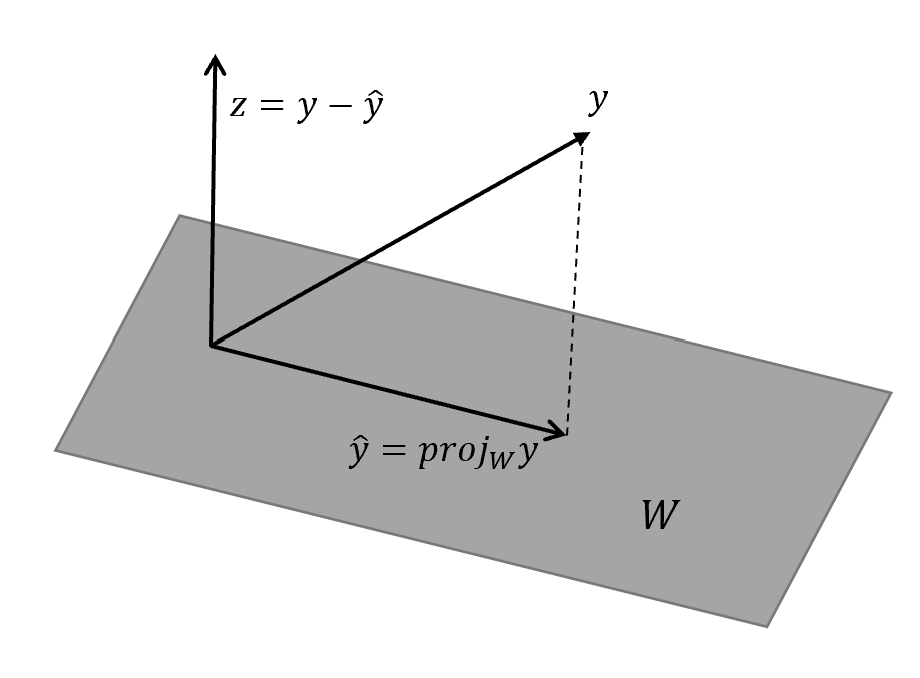
\includegraphics[width = 0.5\textwidth]{Auxiliary Files/Perp Proj.png} }\end{center}
\textbf{Definition} Two vectors $\bm{u}, \bm{v}$ are defined in an inner vector space, where $\bm{u} \cap \bm{v} = \{\bm{0}\}$. Then $\bm{u}$ can be uniquely decomposed into
\begin{equation}
    \bm{u} = \hat{\bm{u}} + \bm{z} = \alpha \bm{v} +  \bm{z} =  \text{proj}_{\bm{Span}\{\bm{v}\}}\bm{u} + \bm{z}
\end{equation}
where $\bm{z} \in (\bm{Span}\{\bm{v}\})^{\perp}$, and $\alpha \bm{v}$ is called the \textbf{orthogonal projection} of $\bm{u}$ on $\bm{Span}\{\bm{v}\}$. The coefficient $\alpha$ can be calculated as
\begin{equation}
    \langle \bm{u},\bm{v}\rangle = \alpha \langle \bm{v},\bm{v}\rangle + \langle \bm{z} , \bm{v} \rangle = \alpha \langle \bm{v},\bm{v}\rangle~~\rightarrow~~\alpha = \frac{\langle \bm{u},\bm{v} \rangle}{\langle \bm{v}.\bm{v}\rangle },~\text{proj}_{\bm{Span}\{\bm{v}\}}\bm{u} = \frac{\langle \bm{u},\bm{v} \rangle}{\langle \bm{v}.\bm{v}\rangle } \bm{v}
\end{equation}\par \noindent 
\textbf{Corollary 10.4.1} For an inner product space $W$, if an orthogonal basis $w = \{\bm{w_1},\bm{w_2},\dots, \bm{w_p} \}$ sufficiently generates it, then if every single orthogonal basis corresponds to the columns of matrix $P$, then
\begin{gather}
    \forall \bm{y} \in W,~~\bm{y} = P[\bm{y}]_{w} = \sum_{i=1}^{p}c_i \bm{w_i} \notag\\
    \text{For}~1 \leq j \leq p,~\langle \bm{w_j}, \bm{y} \rangle = \langle \bm{w_j}, \sum_{i=1}^p c_i \bm{w_i} \rangle = c_j \langle \bm{w_j}, \bm{w_j} \rangle 
\end{gather}
Thus
\begin{equation}
    c_j = \frac{\langle \bm{w_j},\bm{y} \rangle}{\langle \bm{w_j},\bm{w_j}\rangle }
\end{equation}
Without loss of generality, we can conclude that any vector $\bm{y}$ in an inner product space $W$ with an arbitrary orthogonal basis $\beta$ can be interpreted as
\begin{equation}
    \beta = \{\bm{w_1},\bm{w_2},\dots,\bm{w_p}\},~\bm{y}\notin W ~ \rightarrow~\hat{\bm{y}} = \sum_{i=1}^p \text{proj}_{\bm{Span}\{\bm{w_i}\}}\bm{y}
\end{equation}
A more generalized expression is:
\begin{equation}
    \text{proj}_{\bm{Span}\{\bm{w_1},\bm{w_2},\dots,\bm{w_p}\}}\bm{y} = \sum_{i=1}^p\text{proj}_{\bm{Span}\{\bm{w_i}\}} \bm{y}
\end{equation}
\subsection{Gram-Schmidt Orthogonalization}
For an inner product space $W$, assume that $\alpha = \{\bm{u_1}, \bm{u_2},\dots, \bm{u_p}\}$ is a basis of $W$. Then we generate an orthogonal basis $\beta = \{\bm{v_1}, \bm{v_2},\dots, \bm{v_p}\}$. Then the orthogonalization for a basis vector $\bm{u_k}$ is 
\begin{equation}
\begin{aligned}
    \bm{v_k} &= \bm{u_k} - \text{proj}_{\bm{Span}\{\bm{v_1},\bm{v_2},\dots,\bm{v_{k-1}}\}} \bm{u_k} \\
    &=\bm{u_k} - \sum_{i=1}^{k-1}\text{proj}_{\bm{Span}\{\bm{v_i}\}} \bm{u_k} \\
    &= \bm{u_k} - \sum_{i=1}^n \frac{\langle \bm{u_k},\bm{v_i}\rangle}{\langle \bm{v_i},\bm{v_i}\rangle } \bm{v_i}
\end{aligned}
\end{equation}
\section{Method of Least Square}
\subsection{Principle}
The method of least square is a standard approach to approximate the solution for \textbf{overdetermined system}. Given a set of collected data $(x_1,y_1),(x_2,y_2),\dots,(x_n,y_n)$, we tend to obtain a generalized form of the solution
\begin{equation}
    y_j = \sum_{i=0}^{k}\beta_if_i(x_j)
\end{equation}
Or
\begin{equation}
    \begin{bmatrix}
    y_1 \\ y_2 \\ \vdots \\ y_n
    \end{bmatrix} = 
    \begin{bmatrix}
    f_0(x_1) & f_1(x_1) & \cdots & f_k(x_1) \\
    f_0(x_2) & f_1(x_2) & \cdots & f_k(x_2) \\
    \vdots & \vdots & \ddots & \vdots \\
    f_0(x_n) & f_1(x_2) & \cdots & f_k(x_n) 
    \end{bmatrix} \begin{bmatrix}
    \beta_0 \\ \beta_1 \\ \vdots \\ \beta_k
    \end{bmatrix}
\end{equation}
Which can be written as
\begin{equation}
    \bm{y} = X\bm{\beta}
\end{equation}
$\bm{y}$ is the \textbf{sample vector}. $X$ is prediction value vector based on every $x$, called the \textbf{design matrix}. $\bm{\beta}$ is the \textbf{parameter vector}. 
\subsection{Solution of Least Square Equation}
The equation (102) is not always consistent (as the system is over-determined). There will be some bias between $\text{Col}X$ and $y$. Then we write (102) as
\begin{equation}
    \bm{y} = X\bm{\beta} + \bm{\epsilon}~\Leftrightarrow~\bm{\epsilon} = \bm{y} - X\bm{\beta}
\end{equation}
We tend to minimize $\Vert \bm{\epsilon} \Vert$. Thus we take 
\begin{equation}
    X\bm{\beta} = \hat{\bm{y}} = \text{proj}_{\text{Col}X} \bm{y}
\end{equation}
$\hat{\bm{y}} \in \text{proj}_{\text{Col}X} \bm{y}$, hence the equation is now consistent. As $\bm{z} = \bm{y} - \hat{\bm{y}} \in (\text{Col}X)^{T}= \text{Nul}X^{T}$
\begin{equation}
    X^{T}(\bm{y}-\hat{\bm{y}}) = X^{T} (\bm{y} - X\bm{\beta}) = \bm{0}~~\rightarrow~~\boxed{X^TX\bm{\beta} = X^T \bm{y}}
\end{equation}
\subsection{Applications}
\subsubsection{Weighted Least Square Method}
Sometimes data pairs have different significance to fitting the curve. Thus we give every pair of data a weight $w_i$ when maximizing the residual.
\begin{equation}
    \bm{\epsilon}' = \begin{bmatrix}
    w_1(y_1 - \hat{y_1}) \\ w_2(y_2 - \hat{y_2}) \\ \vdots \\ w_n(y_n - \hat{y_n}) 
    \end{bmatrix} = \begin{bmatrix}
    w_1 & & & \\
    & w_2 & & \\
    & & \ddots & \\
    & & & w_n 
    \end{bmatrix} \begin{bmatrix}
    y_1 - \hat{y_1} \\ y_2 - \hat{y_2} \\ \vdots \\ y_n - \hat{y_n}
    \end{bmatrix} = W\bm{\epsilon}
\end{equation}
Then to minimize the norm of $\bm{\epsilon}' = \sqrt{\langle \bm{\epsilon}',\bm{\epsilon}'\rangle}$, we solve the equation
\begin{equation}
    WX\bm{\beta} = W\bm{y}~~\rightarrow~~(WX)^T(WX)\bm{\beta} = (WX)^T \bm{y}
\end{equation}
\subsubsection{Lagrange Interpolation}
To approximate a curve, an intuitive choice is to choose polynomials as the basis. For points $(x_1,y_1),(x_2,y_2),\dots,(x_n,y_n)$, we use a homogeneous polynomial
\begin{equation}
    f(x) = \beta_0 + \beta_1x + \dots + \beta_{n-1}x^{n-1}
\end{equation}
Then we build up the matrix equation $X\bm{\beta} = \bm{y}$
\begin{equation}
    \begin{bmatrix}
    1 & x_1 & x_1^2 & \cdots & x_1^{n-1} \\
    1 & x_2 & x_2^2 & \cdots & x_2^{n-1} \\
    \vdots & \vdots & \vdots & \ddots & \vdots \\
    1 & x_n & x_n^2 & \cdots & x_n^{n-1} \\
    \end{bmatrix} \begin{bmatrix}
    \beta_0 \\ \beta_1 \\ \vdots \\ \beta_{n-1}
    \end{bmatrix} = \begin{bmatrix}
    y_1 \\ y_2 \\ \vdots \\ y_n
    \end{bmatrix}
\end{equation}
Applying Cramer's rule,
\begin{equation}
\begin{aligned}
    \beta_i = \frac{\bm{det}X_i(\bm{y})}{\bm{det}X} &= \frac{1}{\prod_{1 \leq i < j \leq n}(x_j - x_i)}\begin{vmatrix}
    1 & x_1 & \cdots & x_1^{i-2} & y_1 & x_1^{i} & \cdots & x_1^{n-1} \\
    1 & x_2 & \cdots & x_2^{i-2} & y_2 & x_2^{i} & \cdots & x_2^{n-1} \\
    \vdots & \vdots & \ddots & \vdots & \vdots & \vdots & \ddots & \vdots \\
    1 & x_n & \cdots & x_n^{i-2} & y_n & x_n^{i} & \cdots & x_n^{n-1} \\
    \end{vmatrix} \\
    &= \frac{1}{\prod_{1 \leq i < j \leq n}(x_j - x_i)} \sum_{j=1}^{n}y_j C_{j,i} = \frac{1}{\prod_{1 \leq i < j \leq n}(x_j - x_i)} \sum_{j=1}^{n}(-1)^{i+j}y_j A_{j,i}
\end{aligned}
\end{equation}
Where $A_{j,i}$ equals to the coefficient of $t^{i-1}$ in
\begin{equation}
\begin{aligned}
    &\begin{vmatrix}
    1 & x_1 & \cdots & x_1^{i-2} & x_1^{i} & x_1^{i+1} & \cdots & x_1^{n-1}\\
    1 & x_2 & \cdots & x_2^{i-2} & x_2^{i} & x_2^{i+1} & \cdots & x_2^{n-1}\\
    \vdots & \vdots & \ddots & \vdots & \vdots & \vdots & \ddots & \vdots \\
    1 & t & \cdots & t^{i-2} & t^{i-1} & t^i & \cdots & t^{n-1} \\
    \vdots & \vdots & \ddots & \vdots & \vdots & \vdots & \ddots & \vdots \\
    1 & x_n & \cdots & x_n^{i-2} & x_n^{i-1} & x_n^{i} & \cdots & x_n^{n-1}\\
    \end{vmatrix} = (-1)^{n-j}\prod_{\substack{1\leq j-1 \\ s < k \leq n}}(x_k-x_s)  \prod_{\substack{1 \leq k \leq n \\ k \neq j}} (t-x_k) \prod_{j+1 \leq s < k \leq n}(x_k-x_s)\\
    &\text{Coef}_t= (-1)^{n-j}\prod_{\substack{1\leq j-1 \\ s < k \leq n}}(x_k-x_s) \prod_{j+1 \leq s < k \leq n}(x_k-x_s)\cdot(-1)^{n-i+1}\mathop{\sum \cdots \sum}\limits_{1 \leq x_{\alpha_1}  \leq \cdots \leq x_{\alpha_{i-1}} \leq n} x_{\alpha_1}x_{\alpha_2}\cdots x_{\alpha_{i-1}}
\end{aligned} \notag
\end{equation}
Actually the polynomial can be written into a simplified form that
\begin{equation}
    f(x) = \sum_{i=0}^{n-1}\beta_{i}x^{i} = \sum_{i=1}^{n} y_i \prod_{\substack{1 \leq j \leq n \\ j \neq i }} \frac{(x-x_j)}{(x_i - x_j)}
\end{equation}
\subsubsection{Fourier Series}
\noindent \textbf{Lemma} For $n \geq 1$, the following set 
\begin{equation}
    \mathcal{F} = \{ 1, \text{cos}t, \text{cos}2t ,\dots,\text{cos}nt,\text{sin}t,\text{sin}2t,\dots,\text{sin}nt\} \notag
\end{equation}
is an orthogonal set under inner product
\begin{equation}
    \langle f , g\rangle = \int^{2\pi}_{0}f(t)g(t)\text{d}t \notag
\end{equation}
\noindent \textbf{Proof}
\begin{gather}
    \langle \text{cos}at , \text{cos}bt \rangle = \int_{0}^{2\pi}
    \frac{\text{cos}(a-b)t + \text{cos}(a+b)t}{2}\text{d}t = 0 \notag \\
    \langle \text{cos}at , \text{sin}bt \rangle = \int_{0}^{2\pi}
    \frac{\text{sin}(b+a)t + \text{sin}(b-a)t}{2}\text{d}t = 0 \notag
\end{gather}
for $a \neq b$ \hfill $\blacksquare$ \par \noindent
Then $\mathcal{F}$ is an orthogonal basis of a subspace $W$ in $C[0,2\pi]$. The \textbf{optimal approximation} of an arbitrary function $f$ is
\begin{equation}
    f(t) = a_0 + \sum_{m=1}^n (a_m \text{cos}mt + b_m \text{sin}mt )
\end{equation}
where
\begin{equation}
    a_m = \frac{\langle f, \text{cos}mt \rangle}{\langle \text{cos}mt,\text{cos}mt \rangle},~~b_m = \frac{\langle f, \text{sin}mt \rangle}{\langle \text{sin}mt,\text{sin}mt \rangle}
\end{equation}
(108) is called the \textbf{Fourier series} of $f(t)$.
\section{Jacobian Matrix}
If there are two coordinate systems with mapping relationship between basis
\begin{gather}
    \alpha = \{x_1,x_2,\dots,x_n\}~\xrightarrow{f:~\mathbb{R}^n \mapsto \mathbb{R}^n} \beta = \{y_1,y_2,\dots,y_n\} \\
    \text{or}~~~y_i = f_{i}(x_1,x_2,\dots,x_n)
\end{gather}
Then the relationship between the infinitesimals correspond to the basis are
\begin{equation}
    \text{d}\bm{y_i} = \sum_{i=1}^n \frac{\partial f_i}{\partial x_j}\text{d}\bm{x_j}
\end{equation}
or
\begin{equation}
\begin{aligned}
    \begin{bmatrix}
    \text{d}y_1 \\  \text{d}y_2 \\  \vdots \\  \text{d}y_n
    \end{bmatrix} = \begin{bmatrix}
    \sum_{i=1}^n \frac{\partial f_{1}}{\partial x_i} \text{d}x_i  \\  \sum_{i=1}^n \frac{\partial f_{2}}{\partial x_i} \text{d}x_i \\  \ddots \\ \sum_{i=1}^n \frac{\partial f_{n}}{\partial x_i} \text{d}x_i
    \end{bmatrix} 
    = \begin{bmatrix}
    \frac{\partial f_{1}}{\partial x_1} & \frac{\partial f_{1}}{\partial x_2} & \cdots & \frac{\partial f_{1}}{\partial x_n} \\
    \frac{\partial f_{2}}{\partial x_1} & \frac{\partial f_{2}}{\partial x_2} & \cdots & \frac{\partial f_{2}}{\partial x_n} \\
    \vdots & \vdots & \ddots & \vdots \\
    \frac{\partial f_{n}}{\partial x_1} & \frac{\partial f_{n}}{\partial x_2} & \cdots & \frac{\partial f_{n}}{\partial x_n}
    \end{bmatrix} \begin{bmatrix}
    \text{d}x_1\\  \text{d}x_2 \\ \vdots  \\  \text{d}x_n
    \end{bmatrix}
\end{aligned}
\end{equation}
\rule{\textwidth}{0.3mm} \par
\textbf{Lemma 1} Assume that a geometry body in the space spanned by basis $\{\bm{x_1}, \bm{x_2}, \dots, \bm{x_n}\}$, and the linear transformation depicted by $n\times n$ matrix $A$ transforms the basis into $\{y_1,y_2,\dots,y_n\}$, i.e.
\begin{equation}
    A \begin{bmatrix}
    \bm{x_1} & \bm{x_2} & \cdots & \bm{x_n}
    \end{bmatrix} =\begin{bmatrix}
    \bm{y_1} & \bm{y_2} & \cdots & \bm{y_n}
    \end{bmatrix}
\end{equation}
determines new coordinates $y_1, y_2, \dots, y_n$. The magnitude of geometry body determined by new coordinates is
\begin{equation}
    V_{\mathcal{Y}} = |\bm{det}A| V_{\mathcal{X}}
\end{equation}
\textbf{Proof} For each vector in the original space, we have
\begin{equation}
    \bm{u} = c_1\bm{x_1} + c_2 \bm{x_2} + \cdots + c_n\bm{x_n} 
\end{equation}
Then the magnitude to the geometry body depicted by vectors $\bm{u_1}, \bm{u_2}, \dots, \bm{u_n}$ is
\begin{equation}
    \bm{det}\begin{bmatrix}
    \bm{u_1} & \bm{u_2} & \cdots & \bm{u_n}
    \end{bmatrix} 
\end{equation}
For the transformed vector, we have
\begin{equation}
    \bm{u}' = c_1\bm{y_1} + c_2 \bm{y_2} + \cdots + c_n\bm{y_n} = c_1A\bm{x_1} + c_2A\bm{x_2} + \cdots + c_nA\bm{x_n} = A(c_1\bm{x_1} + c_2 \bm{x_2} + \cdots + c_n\bm{x_n} ) 
\end{equation}
Then the new geometry body has the magnitude
\begin{equation}
\begin{aligned}
    \bm{det} \begin{bmatrix}
    \bm{u_1}' & \bm{u_2}' & \cdots & \bm{u_n}' \end{bmatrix} &= \bm{det} \begin{bmatrix}
    A\bm{u_1} & A\bm{u_2} & \cdots & A\bm{u_n}
    \end{bmatrix} = \bm{det} A\begin{bmatrix}
    \bm{u_1} & \bm{u_2} & \cdots & \bm{u_n}
    \end{bmatrix} \\
    &=(\bm{det}A)(\bm{det}\begin{bmatrix}
    \bm{u_1} & \bm{u_2} & \cdots & \bm{u_n}
    \end{bmatrix})\notag~~~~~~~~~~~~~~~~~~~~~~~~~~~~~~~~~~~~~~~~~~~\blacksquare
\end{aligned}
\end{equation}
\rule{\textwidth}{0.3mm}
Then the relationship between the magnitude of the infinitesimal geometry body is
\begin{equation}
    \Omega_y = \left|\begin{vmatrix}
    \frac{\partial f_{1}}{\partial x_1} & \frac{\partial f_{1}}{\partial x_2} & \cdots & \frac{\partial f_{1}}{\partial x_n} \\
    \frac{\partial f_{2}}{\partial x_1} & \frac{\partial f_{2}}{\partial x_2} & \cdots & \frac{\partial f_{2}}{\partial x_n} \\
    \vdots & \vdots & \ddots & \vdots \\
    \frac{\partial f_{n}}{\partial x_1} & \frac{\partial f_{n}}{\partial x_2} & \cdots & \frac{\partial f_{n}}{\partial x_n}
    \end{vmatrix}\right| \Omega_x = |\bm{det}\mathbb{J}| \Omega_x
\end{equation}
Where $\mathbb{J}$ is called the \textbf{Jacobian Matrix}. It depicts the scaling coefficient between two infinitesimals in different coordinates.
\section{Symmetric Matrix}
\subsection{Concept}
If a matrix $A$ satisfies
\begin{equation}
    A = A^T
\end{equation}
then it is called a \textbf{symmetric matrix}.
\subsection{Orthogonality of Eigenvectors}
\noindent \boxed{\text{The set of the eigenvectors of a symmetric matrix is an orthogonal set.}} \par \noindent 
\textbf{Proof} Assume that $\bm{v_1}, \bm{v_2}, \dots, \bm{v_n}$ are eigenvectors of symmetric matrix $A$, and correspond to eigenvalues $\lambda_1,\lambda_2,\dots,\lambda_n$. Then
\begin{gather}
    \forall~\lambda_i,\lambda_j,~~A\bm{v_i} = \lambda_i\bm{v_i},~A\bm{v_j} = \lambda_j \bm{v_j} \notag \\
    \lambda_i\bm{v_i}^T = \bm{v_j}^T A^T~\rightarrow~\lambda_i \bm{v_i}^T \bm{v_j} = \bm{v_i}^T A^T\bm{v_j} = \bm{v_i}^T A\bm{v_j} = \lambda_j \bm{v_i}^T \bm{v_j}
\end{gather}
As $\lambda_i \neq \lambda_j$, we have
\begin{equation}
    \bm{v_i}^T \bm{v_j} = \langle \bm{v_i} , \bm{v_j} \rangle = 0
\end{equation}
which indicates that any two eigenvectors in the set are mutually orthogonal. Also we can conclude that the eigenvectors form an orthogonal basis of the column space determined by matrix $A$. \hfill $\blacksquare$ \par \noindent
\subsection{Orthogonal Diagonalization}
We tend to find the diagonalization of matrix $A$, i.e.
\begin{equation}
    A = P\Lambda P^{-1}
\end{equation}
With the eigenvectors forming the columns of matrix $P$. If we unitize each eigenvector to obtain an orthonormal basis $\{\bm{u_1}, \bm{u_2}, \dots, \bm{u_n} \}$, $\bm{u_i} = \bm{v_i} / \sqrt{\langle \bm{v_i},\bm{v_i} \rangle}$, then we denote the new matrix as $Q$, where $QQ^T = 1$. We have
\begin{equation}
    \boxed{A = Q\Lambda Q^{-1} = Q\Lambda Q^T}~\rightarrow~A^T = (Q\lambda Q^T)^T = Q\Lambda Q^T = A
\end{equation}
Thus the diagonalization is well-defined.
\subsection{Spectral Decomposition}
The diagonalization above gives
\begin{equation}
    A = \begin{bmatrix}
    \bm{u_1} & \bm{u_2} & \cdots & \bm{u_n}
    \end{bmatrix} \begin{bmatrix}
    \lambda_1 & & & \\ & \lambda_2 & &  \\ & & \ddots & \\ & & & \lambda_n \\
    \end{bmatrix} \begin{bmatrix}
    \bm{u_1}^T \\ \bm{u_2}^T \\ \vdots \\ \bm{u_n}^T
    \end{bmatrix} = \sum_{i=1}^n \lambda_i \bm{u_i} \bm{u_i}^T
\end{equation}
\subsection{Singular Value Decomposition (SVD)}
\subsubsection{Derivation}
We are interested in building up a generalized decomposition for an arbitrary $m \times n $ matrix $A$. Notice that $(A^TA)^T = A^T (A^T)^T = A^TA$, which indicates that $A^TA$ itself is a symmetric matrix. Then we apply EVD to $A^TA$.  \par 
Assume that $A^TA = Q \Lambda Q^{T}$, with $\bm{rank}(A) = k$, so the eigenvectors set $q = \{\bm{v_1}, \bm{v_2}, \dots, \bm{v_k} \}$ forms an orthonormal basis for $Q$, then 
\begin{equation}
    \forall~\bm{v_1}, \bm{v_2}~\in~q, ~~\langle A\bm{v_i} , A\bm{v_j} \rangle = (A\bm{v_j})^T A\bm{v_i} = \bm{v_j}^T A^T A \bm{v_i} = \bm{v_j}^T \lambda_i \bm{v_i} = \lambda_i \bm{v_j}^T \bm{v_i} = \lambda_i \langle \bm{v_i}, \bm{v_j} \rangle = 0 \notag
\end{equation}  
So the set $q' = \{ A\bm{v_1}, A\bm{v_2}, \dots, A\bm{v_k} \}$ is also orthogonal. Assume that the vectors in $q$ forms the columns of matrix $V$, then
\begin{equation}
    AV = A\begin{bmatrix} \bm{v_1} & \bm{v_2} & \cdots & \bm{v_k} \end{bmatrix}
    = \begin{bmatrix} A\bm{v_1} & A\bm{v_2} & \cdots & A\bm{v_k} \end{bmatrix}
\end{equation}
If we normalize $q'$,  i.e. $\bm{u_i} = A\bm{v_i} / \sqrt{\langle A\bm{v_i}, A\bm{v_i} \rangle}  = A\bm{v_i} / \sqrt{\lambda_i}$, then we denote the singular value $\sigma_i = \sqrt{\lambda_i}$ and obtain
\begin{equation}
    A\bm{v_i} = \sigma_i \bm{u_i}~\leftrightarrow~A\begin{bmatrix} \bm{v_1} & \bm{v_2} & \cdots & \bm{v_k} \end{bmatrix} = \begin{bmatrix} \sigma_1 & & & \\
        & \sigma_2 & & \\ & & \ddots & \\ &&& \sigma_k \end{bmatrix} \begin{bmatrix}
    \bm{u_1} & \bm{u_2} & \cdots & \bm{u_k} \end{bmatrix} 
\end{equation}
We use $U$ and $\Sigma$ to denote the two matrices on the RHS respectively, and thus we conclude that
\begin{equation}
    AV = U\Sigma~\rightarrow~\boxed{A = U\Sigma V^T = \sum_{i=1}^k \sigma_i \bm{u_i}\bm{v_i}^T}
\end{equation}
The product on the RHS shows the \textbf{singular value decomposition} of an arbitrary matrix $A$.
If we expand the set $\{\bm{u_1}, \bm{u_2}, \dots, \bm{u_k}\}$ and $\{\bm{v_1}, \bm{v_2}, \dots, \bm{v_k}\}$ to form a basis of $\mathbb{R}^n$ and $\mathbb{R}^n$ respectively, we then obtain
\begin{equation}
    A = \begin{bmatrix}
        \begin{array}{cccc|ccc}
            \bm{u_1} & \bm{u_2} & \cdots & \bm{u_k} & \bm{u_{k+1}} & \cdot & \bm{u_{n}}
        \end{array}
    \end{bmatrix} \begin{bmatrix} \begin{array}{cccc|c} \sigma_1 & & & & \\
        & \sigma_2 & & & \bm{0} \\
        & & \ddots & & \\ & & & \sigma_k & \\ \hline 
        & & \bm{0} & & \bm{0}
    \end{array} \end{bmatrix} \begin{bmatrix}
        \bm{v_1}^T \\ \bm{v_2}^T \\ \vdots \\ \bm{v_k}^T \\\hline \\ \bm{v_{k+1}}^T \\ \vdots \\ \bm{v_m}^T
    \end{bmatrix}
\end{equation}
\subsubsection{Application}
\end{document}